\documentclass{../../template/mai_book}

\defaultfontfeatures{Mapping=tex-text}
\setmainfont{DejaVuSerif}
\setdefaultlanguage{russian}

% === move to mai_book.cls===
\usepackage{caption}
\usepackage[justification=centering]{caption}
\usepackage[labelsep=period]{caption}
\usepackage{mathtools}
\DeclarePairedDelimiter{\abs}{\lvert}{\rvert}
\DeclarePairedDelimiter{\floor}{\lfloor}{\rfloor}
% ===========================

\begin{document}

\lhead{\small\textit{Решения упражнений}}
\rhead{145}

\noindent
[1, $n$] в [1, $n$], при этом коэффициент $\mu_\alpha$ определяется суммой

\begin{equation*}
\mu_{\alpha} = \sum_{\epsilon_i\in\{0,1\}} (-1)^{\epsilon_1+...+\epsilon_n} \epsilon_{\alpha(1)}...\epsilon_{\alpha(n)}.
\end{equation*}

\noindent
Если $\alpha$ — перестановка, коэффициент $\mu_\alpha$ равен $(—1)^n$, поскольку единственный ненулевой член суммы — это тот, для которого все $\epsilon_i$, равны 1. В противном случае можно разложить $\mu_\alpha$ следующим образом:

\begin{equation*}
\sum_{\epsilon_i, i \neq k} (-1)^{\epsilon_1+...+\epsilon_n} \sum_{\epsilon_k=0,1} (-1)^{\epsilon_k} \epsilon_{\alpha(1)}...\epsilon_{\alpha(n)},
\end{equation*}

\noindent
где $k$ — элемент из [1, $n$], который не принадлежит образу $\alpha$, и хорошо видно, что внутренний член (сумма по $\epsilon_k$) равен нулю; это доказывает, что $\mu_\alpha$ в этом случае равно нулю. Второе искомое выражение (суммы которого записываются на множествах) просто выводится из первого, исключением ненулевых $\epsilon_i$, появляющихся в сумме.

\setcounter{lstlisting}{11}
\captionsetup[lstlisting]{labelfont={bf}}

\begin{wrapfigure}{r}{7cm}
\begin{lstlisting} [language=C,
					basicstyle=\small,
					linewidth=7cm, 
					belowskip=-1em,
					mathescape=true, 
					caption=Вычисление перманента]
S[1] = a[1][succ($n$)]; P = S[1];
for (int i = 2; i <= n; ++i)
	S[i] = a[i][succ($n$)]; P *= S[i];
$\sum$ = -P; E = succ($n$);
while (E != E$_{max}$) {
	j = E $\Delta$ E$^{'}$; S[1] $\pm$= a[1][j];
	P = pow(-1, abs(E$^{'}$)) * S[1];
	for (int i = 2; i <= n; ++i)
		S[i] $\pm$= a[i][j]; P *= S[i];
	$\sum$ += P; E = E$^{'}$;
}
return pow(-1, n) * $\sum$;
\end{lstlisting}
\end{wrapfigure}

\subparagraph{b.} Возвратный код Грея из $n$ разрядов является выражением линейного порядка на множестве всех частей $E$ из [1, $n$], наименьший элемент которого есть 0̸  и наибольший, $E_{max}$, исходное множество. Если $E'$ является последователем для $E$, то симметрическая разность $E \Delta E'$ сводится к одному элементу, а это означает, что $E'$ получается, исходя из $E$, добавлением или удалением одного элемента. Введем несколько обозначений: $E'$ = succ($E$), ${\sum}_E = {\sum}_{F \leqslant E} (-1)^{\abs{F}} {\prod}_{1 \leqslant i \leqslant n} S_i (F)$, где $S_i (E) = {\sum}_{j \in E} a_{ij}$. Вычисляемый перманент является, значит, суммой $(-1)^n {\sum}_{E_{max}}$. Эта сумма получается вычислением последовательных значений ${\sum}_E$ и, тогда, итерируя, имеем:

\setcounter{equation}{6}

\begin{equation}
{\sum}_{E'} = {\sum}_E + (-1)^{|E'|} \prod_{1 \leqslant i \leqslant n} S_i(E').
\end{equation}

\noindent
Вклад наименьшего элемента 0̸  в эту сумму — нулевой; значит, начнем с его последователя, который может быть \{1\}, \{$n$\} или какое-нибудь одноэлементное множество в соответствии с порядком, заданным на [1, $n$]. Можно заметить, что $S_i(E') = S_i(E) \pm a_{ij}$, где $\{j\} = E \triangle E'$.

\newpage

\lhead{146}
\rhead{\small\textit{$I$ \quad Алгоритмика и программирование на языке Ада}}

\noindent
В этой записи, как в алгоритме 12, $\pm$ должен пониматься как $+$, если $E \subset E'$ и $-$, если $E' \subset E$.

Чтобы оценить ${\sum}_{E'}$, исходя из ${\sum}_E$ с использованием 
соотношения (7), нужно осуществить $n$ сложений (для подсчета каждого $S_i (E')$), затем $n - 1$ перемножений: $S_1(E') \times \cdots \times S_n(E')$, и, наконец, 1 сложение. Имеем $2^n - 2$ операций для осуществления (7), при этом первый член $\sum = -{\prod}_{1 \leqslant i \leqslant n} \alpha_{in}$ требует $n - 1$ перемножений; это доказывает сформулированный результат о сложности. Сложность \textit{O}($n2^n$) значительна, но остается того же порядка, что и сложность, индуцированная определением ($n!(n - 1)$ перемножений и $n! - 1$ сложений). Формула Стирлинга позволяет сравнить эти два значения сложности: $ n \cdot n!/(n \cdot 2^n) \approx (n/2e)^n \sqrt{2\pi n}$.

\paragraph{22. Перманент матрицы (продолжение)}

\subparagraph{a.} Правая часть может рассматриваться как многочлен (от переменных $a_{ij}$), равный ${\sum}_\alpha \mu_\alpha a_{1 \alpha(1)} ... a_{n \alpha(n)}$, где сумма распространяется на все отображения [1, $n$] в [1, $n$]. Коэффициент $\mu_\alpha$ задан формулой

\begin{equation*}
\mu_\alpha = \sum_\omega \mu_\alpha(\omega) \quad \text{с} \quad \mu_\alpha(\omega) = \omega_1 \text{ ... } \omega_{n - 1} \omega_{\alpha(1)} \text{ ... } \omega_{\alpha(n)},
\end{equation*}

\noindent
в которой полагаем $\omega_n = 1$. Если $\alpha$ — перестановка, то каждое $\mu_\alpha(\omega)$, присутствующее в сумме $\mu_\alpha$, равно 1 и, следовательно, $\mu_\alpha = 2^{n - 1}$. Напротив, если $\alpha$ не является перестановкой, то сумма $\mu_\alpha$ — нулевая. Действительно, образ $\alpha$ отличен от [1, $n$], и различаем два случая: \newline
\indent ($i$) $\exists$ $k < n$, не принадлежащий образу $\alpha$, \newline
\indent ($ii$) $\exists$ $k < n$, дважды полученный из $\alpha$.

В обоих случаях члены $\mu_\alpha(\omega)$, присутствующие в сумме, группируются попарно, один соответствуя $\omega_k = 1$, другой — $\omega_k = -1$, и взаимно уничтожаются (в случае ($ii$) $\mu_\alpha(\omega) = \omega_k$).

\subparagraph{b.} Формула пункта \textbf{a} может быть записана в следующем виде:

\begin{equation*}
\frac{per A}{2} = \sum \omega_1 \text{ ... } \omega_{n - 1} \prod_{1 \leqslant i \leqslant n} (a_{in} + \omega_1 a_{i1} + \cdots + \omega_{n - 1} a_{in - 1})/2.
\end{equation*}

\noindent
Как и в предыдущем упражнении, вычисление перманента получается генерированием перебора при линейной упорядоченности на $\{-1, 1\}^{n - 1}$, в которой два последовательных элемента отличаются только одной компонентой. Если для $\omega \in \{-1, 1\}^{n - 1}$ и $i \leqslant n$ положить

\begin{equation*}
S_i(\omega) = (a_{in} + \omega_1 a_{i1} + \cdots + \omega_{n - 1} a_{in - 1})/2,
\end{equation*}

\newpage

\lhead{\small\textit{Решения упражнений}}
\rhead{147}

\noindent
то можно, благодаря перебору на $\{-1, 1\}^{n - 1}$, вычислить последовательно ${\sum}_\omega = {\sum}_{\rho \leqslant \omega}$... , используя формулу

\begin{equation}
	\begin{split}
	{\sum}_{\omega'} \quad = \quad &{\sum}_\omega + {\omega'}_1 \text{ ... } {\omega'}_{n - 1} \prod_{1 \leqslant i \leqslant n} S_i(\omega'),
	\\
	&\text{где } \omega' \text{ — последователь для } \omega \text{ в } \{-1, 1\}^{n - 1}.
	\end{split}
\end{equation}

\noindent
Если $j$ является индексом, по которому различаются два слова $\omega$ и $\omega'$, то сумма $S_i(\omega')$ вычисляется, исходя из $S_i(\omega)$, через $S_i(\omega') = S_i(\omega) - a_{ij}$, если $\omega_j = 1$, и через $S_i(\omega') = S_i(\omega) + a_{ij}$, если $\omega_j = -1$.

\renewcommand{\figurename}{Алгоритм}

\begin{figure}[htp]
\centering
\begin{tabular}{c}
\begin{lstlisting} [language=C,
					basicstyle=\small,
					linewidth=9.3cm, 
					mathescape=true, 
					caption=Вычисление перманента в кольце\, где 2 обратимо]
for (int i = 1; i <= n; ++i)
	S[i] = (a[i][1] + ... + a[i][n]) / 2;
$\sum$ = S[1] * ... * S[n]; $\epsilon$ = {0, ..., 0}; sgn = 1;
while ($\epsilon$ != $\epsilon_{max}$) {
	$\epsilon^{'}$ = succ($\epsilon$); sgn = -sgn; j = $\epsilon$ $\Delta$ $\epsilon^{'}$;
	if ($\epsilon_j$ == 0)
		for (int i = 1; i <= n; ++i)
			S[i] -= a[i][j];
	else // $\epsilon_j$ == 1
		for (int i = 1; i <= n; ++i)
			S[i] += a[i][j];
	$\sum$ += sgn * S[1] * ... * S[n]; $\epsilon$ = $\epsilon^{'}$;
}
return 2 * $\sum$;
\end{lstlisting}
\end{tabular}
\end{figure}

\textbf{Алгоритм 13.} Вычисление перманента в кольце, где 2 обратимо \newline

С практической точки зрения для генерации адекватного перебора \linebreak $\{-1, 1\}^{n - 1}$, выбираем соответствие между $\{0, 1\}$ и $\{-1, 1\}$ вида $\epsilon \mapsto (-1)^\epsilon$ и классическую генерацию кода Грея на $\{0, 1\}^{n - 1}$, что достигается с помощью алгоритма 13. Мультипликативная сложность получается, если заметить, что нужно вычислить $2^n - 1$ членов ${\sum}_\omega$ , каждый из которых требует $n - 1$ перемножений (см. формулу (8)), значит, всего $2^{n - 1}(n - 1)$ произведений, к которым нужно добавить последнее умножение на 2. С точки зрения сложений первоначальный член ${\sum}_{(1,...,1)}$ требует $n(n - 1)$ сложений и $n$ делений на 2, тогда как общий член ${\sum}_\omega$ вычисляется, исходя из предыдущего, с помощью $n$ сложений; наконец, нужно сложить все эти члены, что требует в целом $n(n - 1) + (2^{n - 1} - 1)(n + 1)$ сложений и $n$ делений на 2. Заметим относительно предыдущего упражнения, что сложность была приблизительно разделена на 2.

\newpage

\lhead{148}
\rhead{\small\textit{$I$ \quad Алгоритмика и программирование на языке Ада}}

\subparagraph{c.} Рассмотрения полностью аналогичны предыдущему пункту, если
только невозможно деление на 2; деление (точное) на $2^{n - 1}$ будет иметь
место уже в конце. Результатом является алгоритм 14. \newline

\begin{figure}[htp]
\centering
\begin{tabular}{c}
\begin{lstlisting} [language=C,
					basicstyle=\small,
					linewidth=9.3cm, 
					mathescape=true, 
					caption=Вычисление перманента для характеристики\, 							отличной от 2]
for (int i = 1; i <= n; ++i)
	S[i] = a[i][1] + ... + a[i][n];
$\sum$ = S[1] * ... * S[n]; $\epsilon$ = {0, ..., 0}; sgn = 1;
while ($\epsilon$ != $\epsilon_{max}$) {
	$\epsilon^{'}$ = succ($\epsilon$); sgn = -sgn; j = $\epsilon$ $\Delta$ $\epsilon^{'}$;
	if ($\epsilon_j$ == 0)
		for (int i = 1; i <= n; ++i)
			S[i] -= 2 * a[i][j];
	else // $\epsilon_j$ == 1
		for (int i = 1; i <= n; ++i)
			S[i] += 2 * a[i][j];
	$\sum$ += sgn * S[1] * ... * S[n]; $\epsilon$ = $\epsilon^{'}$;
}
return $\sum$/($2^{n - 1}$);
\end{lstlisting}
\end{tabular}
\end{figure}

\paragraph{23. Массив инверсий подстановки}

\subparagraph{d.} Массив инверсий перестановки $\alpha$ имеет вид (0, 0, 0, 1, 4, 2, 1, 5, 7). Свойство $0 \leqslant \alpha_k < k$ легко получается из того, что имеется точно $k - 1$ целых чисел, заключенных строго между 0 и $k$. Массив инверсий возрастающей перестановки интервала [1, $n$] есть, очевидно, (0, 0, ... , 0), и таблица для единственной убывающей перестановки —  (0, 1, 2, ... , n).

\subparagraph{e.} Можно использовать тот факт, что $a_{\alpha(j)}$ есть число индексов таких, что $i > j$ и $\alpha(i) < \alpha(j)$, что приводит к нижеследующему алгоритму:

\begin{leftbar}
\begin{lstlisting} [language=C,
					basicstyle=\small,
					linewidth=6.8cm, 
					mathescape=true, 
					frame=none]
{ a[1], ..., a[n] } = { 0, ..., 0 }
for (int j = 1; j <= n; ++j)
	for (int i = j + 1; i <= n; ++i)
		if ($\alpha$(i) < $\alpha$(j))
			a[$\alpha$(j)]++; 
\end{lstlisting}
\end{leftbar}

Сложность полученного способа, конечно, имеет порядок квадрата длины перестановки.

\newpage

\lhead{\small\textit{Решения упражнений}}
\rhead{149}

\subparagraph{f.} Пусть $a$ — элемент из $[0, 1[ \times [0, 2[ \times \cdots \times [0, n[$. Построим перестановку $\alpha$, для которой $a$ является массивом инверсий, следующим способом: \newline

$\bullet$ элемент $n$ помещаем в массив, индексированный с помощью [1, $n$], представляющий $\alpha$, оставляя $a_n$ \textbf{пустых ячеек} справа от $n$; это означает в точности, что $\alpha^{-1}(n) = n - a_n + 1$;

$\bullet$ затем помещаем $n - 1$ в массив $\alpha$, оставляя $\alpha_{n - 1}$ \textbf{пустых ячеек} справа от $n - 1$;

$\bullet$ продолжаем, зная, что на $k$-м этапе этого процесса $k - 1$ величин уже размещены в массиве, следовательно, в массиве $\alpha$ остается $n - k$ свободных мест, и, с другой стороны, величина $\alpha_{n - k}$ строго меньше, чем $n - k$. \newline

\noindent
\begin{figure}[htp]
\centering
\begin{tabular}{c}
\begin{lstlisting} [language=C,
					basicstyle=\small,
					linewidth=7cm, 
					mathescape=true, 
					caption=Генерация перестановок]
{ $\alpha$[1], ..., $\alpha$[n] } = { 1, ..., 1 }
for (int k = 2; k <= n; ++k) {
	j = n; i = 0;
	do {
		if (a$_j$ == 1) // (#1)
			i++;
		j--;
	} while (i != 1 + a$_k$); // (#2)
	$\alpha_{j + 1} = k;$
}
\end{lstlisting}
\end{tabular}
\end{figure}

\begin{leftbar}
\noindent
\#1: \quad $i$ есть число свободных индексов > $j$
\\
\#2: \quad $i$ = 1 + a$_k$, то $j$ свободен
\end{leftbar}

В алгоритме 15 использована оптимизация: свободные места в массиве, представляющем перестановку $\alpha$, отмечены числами 1, что позволяет не помещать это последнее значение в массив, представляющий $\alpha$, в конце алгоритма.

\paragraph{24. Перебор перестановок транспозициями $(i, i + 1)$}

\subparagraph{a.} Рассуждаем индукцией по $n$, при этом случаи $n = 1$ и $n = 2$ очевидны. С помощью перестановки $\sigma$ интервала [1, $n$] можно построить $n + 1$ перестановок $\sigma^1, \sigma^2, \text{ ... } , \sigma^{n + 1}$ интервала [1, $n + 1$], где перестановка $\sigma^i$ получается включением в $\sigma$ элемента $n + 1$ на $i$-ое место; например, если \linebreak

\newpage

\lhead{150}
\rhead{\small\textit{$I$ \quad Алгоритмика и программирование на языке Ада}}

\noindent
$\sigma$ = (5 2 4 1 3), то

\begin{equation*}
	\begin{split}
	\sigma^1 &= \text{(\underline{6} 5 2 4 1 3)}, \quad \sigma^2 = \text{(5 \underline{6} 2 4 1 3), ... ,}
	\\
	&\sigma^5 = \text{(5 2 4 1 \underline{6} 3)}, \quad \sigma^6 = \text{(5 2 4 1 3 \underline{6})}.
	\end{split}
\end{equation*}

\noindent
Если $\sigma_1, \sigma_2, \text{ ... } , \sigma_{n!}$ и есть такая последовательность перестановок на [1, $n$], то соответствующую последовательность перестановок интервала [1, $n + 1$] получаем следующим образом:

\begin{equation*}
	\begin{split}
	&\sigma_1^1, \sigma_1^2, \text{ ... } , \sigma_1^{n + 1}, \quad \sigma_2^{n + 1}, \sigma_2^n, \text{ ... } , \sigma_2^1
	\\
	\sigma_3^1, &\sigma_3^2, \text{ ... } , \sigma_3^{n + 1}, \quad \sigma_4^{n + 1}, \sigma_4^n, \text{ ... }, \sigma_4^1 \quad \text{и т.д.}
	\end{split}
\end{equation*}

\subparagraph{b.} Действуем индукцией по $n$; знаем, что \textit{b} —  последующий элемент для $a$ в знакопеременном лексикографическом порядке —  получается изменением \textit{одной} компоненты $а$. Предположим сначала, что эта компонента — последняя; тогда имеем $b_n = a_n \pm 1$ и $b_j = a_j$ для $1 \leqslant j \leqslant n - 1$. Если $i$ — индекс $n$ в $\alpha$ (т.е. $\alpha(i) = n$), то имеем $\beta = \alpha \circ (i, i - 1)$ в случае $b_n = a_n + 1$, и $\beta = \alpha \circ (i, i + 1)$ в случае $b_n = a_n - 1$, при этом запись $(j, k)$ означает транспозицию индексов j и k.

Теперь предположим, что компонента, по которой различаются $a$ и $b$, не является последней. Поскольку $b$ — последующий элемент для $a$ в знакопеременном лексикографическом порядке, имеем $a_n = b_n = 0$ или $a_n = b_n = n$ и $b_{[1..n - 1]}$ есть последующий элемент для $a_{[1..n - 1]}$ в лексикографическом знакопеременном произведении $[0, 1[ \times [0, 2[ \times \cdots \times [0, n - 1[$, причем компонентой с самым большим индексом массива инверсий является та, которая меняется быстрее всех во время перебора в лексикографическом знакопеременном порядке. Если $\alpha'$ (соответственно, $\beta'$) означает перестановку [1, $n - 1$], для которой $a_{[1..n - 1]}$ (соответственно, $b_{[1..n - 1]}$) массив инверсий, то $\beta'$ получается из $\alpha'$ транспозицией двух последовательных элементов (гипотеза индукции). Тогда утверждение верно также и для $\alpha$ и $\beta$, поскольку элемент $n$ находится в этих перестановках либо на месте $n$ (случай $a_n = b_n = 0$), либо на месте 1 (случай $a_n = b_n = n$).

\subparagraph{c.} Пусть $\alpha$ — перестановка интервала [1, $n$] и $a = (a_1, a_2, \text{ ... }, a_n)$ — ее массив инверсий. По предыдущему сигнатура перестановки $\alpha$ является также сигнатурой $a$ в знакопеременном лексикографическом произведении. Алгоритм вычисления последующего элемента в знакопеременном лексикографическом произведении приводит к алгоритму 16-А.

В начале тела основного цикла этого алгоритма делается попытка опустить элемент $q$ (применить транспозицию ($\alpha^{-1}(q) - 1, a^{-1}(q)$) к перестановке $\alpha$) или же поднять его.

\newpage

\lhead{\small\textit{Решения упражнений}}
\rhead{151}

Фактически, бесполезно приниматься за предварительное вычисление массива инверсий $a$. Достаточно вычислить при необходимости элемент $a_q$, что может быть реализовано одновременно с вычислением $\alpha^{-1}(q)$ благодаря алгоритму 16-В. В этом втором алгоритме результирующим значением $i$ является $\alpha^{-1}(q)$. \newline

\textit{// here goes some code}

\paragraph{25. Принцип включения-исключения или формула решета}

\subparagraph{a.} Первая формула удобно получается индукцией по $\abs{I}$, числу элементов $I$, с использованием хорошо известной формулы $\abs{A \cup B} = \abs{A} + \abs{B} - \abs{A \cap B}$. Вторая получается переходом к дополнениям. Чтобы получить формулу Сильвестра, достаточно записать:

\begin{equation*}
\bigcap_{i \in I} \overline{X_i} = \overline{\bigcup_{i \in I} X_i} = X - \bigcup_{i \in I} X_i,
\end{equation*}

\noindent
затем применить первую формулу.

\subparagraph{b.} Пусть X — множество всех перестановок на [1, $n$] и $X_i$ —  множество перестановок, имеющих $i$ фиксированной точкой, $1 \leqslant i \leqslant n$. Искомое число $\sigma_n$:

\begin{equation*}
\sigma_n = \abs[\Big]{\bigcup_{i \in [1, n]} \overline{X_i}} = \sum_{J \subset [1, n]} (-1)^{\abs{J}} \abs[\Big]{\bigcap_{i \in J} X_i}.
\end{equation*}

\noindent
Множество $\bigcap X_i$ есть множество $J$ перестановок на [1, $n$] и, следовательно, содержит $(n - \abs{J})!$ элементов, откуда:

\begin{equation*}
\sigma_n = \sum_{J \subset [1, n]} (-1)^{\abs{J}} (n - \abs{J})! = \sum_{k = 0}^n (-1)^k C_n^k(n - k)! = \sum_{k = 0}^n (-1)^k \frac{n!}{k!}
\end{equation*}

\newpage

\lhead{152}
\rhead{\small\textit{$I$ \quad Алгоритмика и программирование на языке Ада}}

\subparagraph{c.} Положим здесь $X$ равным интервалу [1, $n$] и для $1 \leqslant i \leqslant k$ пусть $X_i$ — множество элементов из $X$, которые кратны $p_i$. Тогда имеем:

\begin{equation*}
\phi(n) = \abs[\Big]{\bigcap_{i \in [1, k]} \overline{X_i}} = \sum_{J \subset [1, k]} (-1)^{\abs{J}} \abs[\Big]{\bigcap_{i \in J} X_i}
\end{equation*}

\noindent
Множество $\bigcap X_i$ здесь является множеством элементов из X, кратных ${\prod}_{i \in J} p_i$; но если $d$ является делителем $n$, имеется точно $n / d$ элементов из $X$, кратных $d$, откуда:

\begin{equation*}
\phi(n) = n \sum_{J \subset [1, k]} \frac{(-1)^{\abs{J}}}{{\prod}_{i \in J} p_i} = n (1 - \frac{1}{p_1}) (1 - \frac{1}{p_2}) \text{ ... } (1 - \frac{1}{p_k}).
\end{equation*}

\subparagraph{d.} Обозначим через $X$ множество всех отображений из [1, $n$] в [1, $n$] и для $1 \leqslant i \leqslant n$ через $X_i$ — множество отображений из X, не имеющих $i$ в их образе; выберем в качестве весовой функции на $X$ функцию $p(\alpha) = a_{1\alpha(1)} a_{2\alpha(2)} \text{ ... } a_{n\alpha(n)}$: тогда нужно вычислить вес множества $S_n$ всех перестановок на [1, $n$]. Заметим, что $S_n = {\bigcap}_{i \in [1, n]} \overline{X_i}$ и, значит, $per A =$ \linebreak ${\sum}_{J \subset [1, n]} (-1)^{\abs{J}} p({\bigcap}_{i \in J} X_i)$. Но ${\bigcap}_{i \in J} X_i$ есть множество всех отображений, образы которых не встречаются в $J$, следовательно:

\begin{equation*}
p(\bigcap_{i \in J} X_i) = \sum_{\alpha : [1, n] \rightarrow \overline{J}} a_{1\alpha(1)} \text{ ... } a_{n\alpha(n)} = \sum_{j \not\in J} a_{1j} \sum_{j \not\in J} a_{2j} \text{ ... } \sum_{j \not\in J} a_{nj}
\end{equation*}

\noindent
отсюда получаем формулу $per A = {\sum}_{J \subset [1, n]} (-1)^{\abs{J}} {\prod}_{i = 1}^n {\sum}_{j \not\in J} a_{ij}$, которая при замене $J$ его дополнением дает формулу Райзера.

\paragraph{26. Произведение многочленов, заданных массивами} \mbox{}\\

\begin{wrapfigure}{r}{7.5cm}
\begin{lstlisting} [language=C,
					basicstyle=\small,
					linewidth=7.5cm,
					aboveskip=-1em,
					belowskip=-1em,
					mathescape=false,
					frame=l]
					
for (int i = 0; i < arrlen(P); ++i)
	for (int j = 0; j < arrlen(Q); ++j)
		R[i + j] += P[i] * Q[j];
\end{lstlisting}
\end{wrapfigure}

\subparagraph{a.} Алгоритм справа дает \linebreak функцию умножения двух многочленов $Р$ и $Q$, где многочлен $R$ степени deg $P$ + deg $Q$ (который дает результат в конце алгоритма) должен быть предварительно инициализирован нулем. \newline

\subparagraph{b.} Изучая предыдущий алгоритм, устанавливаем, что его сложность, как по числу перемножений, так и сложений, равна произведению высот двух многочленов: (deg $P$ + 1) $\times$ (deg $Q$ + 1) — обычно высотой многочлена \linebreak

\newpage

\lhead{\small\textit{Решения упражнений}}
\rhead{153}

\begin{wrapfigure}{l}{7.8cm}
\begin{lstlisting} [language=C,
					basicstyle=\small,
					linewidth=7.8cm,
					belowskip=-1em,
					mathescape=false,
					caption=Перемножение многочленов]
for (int i = 0; i < arrlen(P); ++i)
	if (P(i) != 0)
		for (int j = 0; j < arrlen(Q); ++j)
			if (Q(j) != 0)
				R[i + j] += P[i] * Q[j]
\end{lstlisting}
\end{wrapfigure}

\noindent
называют число его ненулевых коэффициентов, но в этом алгоритме, который не учитывает случай нулевых коэффициентов, можно рассматривать высоту многочлена как число всех коэффициентов. Значит, возможно улучшить предыдущий алгоритм, исключив все ненужные перемножения: это сделано в алгоритме 17. В противовес тому, что можно было бы подумать, эта оптимизация вовсе не смехотворная и активно применяется при умножении разреженных многочленов.

\paragraph{27. Возведение в степень многочленов, заданных массивами}

\subparagraph{a.} Очень просто вычислить сложность алгоритма возведения в степень последовательными умножениями, если заметить, что когда $P$ — многочлен степени $d$, то $P^i$ — многочлен степени $id$. Если обозначить $C_{mul}(n)$ сложность вычисления $P^n$, то рекуррентное соотношение $C_{mul}(i + 1) =$ \linebreak $C_{mul}(i) + (d + 1) \times (id + 1)$ дает нам:

\begin{equation*}
C_{mul}(n) = (d + 1) \sum_{i = 1}^{n - 1} id + 1 = \frac{n^2 d(d + 1)}{2} + \frac{n(d + 1)(2 - d)}{2} - (d + 1).
\end{equation*}

\subparagraph{b.} Что касается возведения в степень с помощью дихотомии (т.е. повторяющимся возведением в квадрат), вычисления несколько сложнее: зная $P^{2^i}$, вычисляем $P^{2^{i + 1}}$ с мультипликативной сложностью $(2^i d + 1)^2$. Как следствие имеем:

\begin{equation*}
	\begin{split}
	C_{sqr}(2^l) = \sum_{i = 0}^{l - 1} (2^i d + 1)^2 &= \frac{d^2 (4^l - 1)}{3} + 2d(2^l - 1) + l =
	\\
	&= \frac{d^2 n^2}{3} + 2nd + \log_2 n - 2d - \frac{d^2}{3}
	\end{split}
\end{equation*}

\noindent
Предварительное заключение, которое можно вывести из предыдущих вычислений, складывается в пользу дихотомического возведения в степень: если $n$ есть степень двойки (гипотеза ad hoc), этот алгоритм еще выдерживает конкуренцию, даже если эта победа гораздо скромнее в данном \linebreak

\newpage

\lhead{154}
\rhead{\small\textit{$I$ \quad Алгоритмика и программирование на языке Ада}}

\noindent
контексте ($n^2 d^2 / 3$ против $n^2 d^2 / 2$), чем когда работаем в $\mathbb{Z} / p \mathbb{Z}$ ($2 \log_2 n$ против $n$).

Но мы не учли корректирующие перемножения, которые должны быть выполнены, когда показатель не является степенью 2-х. Если $2^{l + 1} - 1$, нужно добавить к последовательным возведениям в квадрат перемножения всех полученных многочленов. Умножение многочлена $P^{(2^i - 1)d}$ степени $(2^i - 1)d$ на многочлен $P^{2^i d}$ степени $2^i d$ вносит свой вклад из $((2^i - 1)d + 1) \times (2^i d + 1)$ умножений, которые, будучи собранными по всем корректирующим вычислениям, дают дополнительную сложность:

\begin{equation*}
	\begin{split}
	C_{sqr}'(2^{l + 1} - 1) &= \sum_{i = 1}^l ((2^i - 1)d + 1) \times (2^i d + 1) =
	\\
	&= \frac{d^2 n^2}{3} - \frac{4d^2 n}{3} + 2nd -2d^2 + d(1 - \floor{\log_2 n} ).
	\end{split}
\end{equation*}

\noindent
Теперь можно заключить, что дихотомическое возведение в степень не всегда является лучшим способом для вычисления степени многочлена с помощью перемножений многочленов. Число перемножений базисного кольца, которые необходимы, $C_{sqr}(n)$ — в действительности заключено между $C_{sqr}(2^{\floor{log_2 n}})$ и $C_{sqr}(2^{\floor{log_2 n}}) + C'(2^{\floor{log_2 n} + 1} - 1)$, т.е. между $n^2 d^2 / 2$ и $2n^2 d^2 / 3$, тогда как простой алгоритм требует всегда $n^2 d^2 / 2$ перемножений. В частности, если исходный многочлен имеет степень, большую или равную 4, возведение в степень наивным методом  требует меньше перемножений в базисном кольце, чем бинарное возведение в степень, когда $n$ имеет форму $2^l - 1$. \newline


Можно пойти еще дальше без лишних вычислений: можно довольно просто доказать, что если $n$ имеет вид $2^l + 2^{l - 1} + c$ (выражения, представляющие двоичное разложение $n$), то метод вычисления последовательными перемножениями лучше метода, использующего возведение в квадрат (этот последний метод требует корректирующего счета ценой, по крайней мере, $n^2 d^2 / 9$). Все это доказывает, что наивный способ является лучшим для этого класса алгоритмов, по крайней мере в половине случаев. \newline

Действительно, МакКарти [124] доказал, что дихотомический алгоритм возведения в степень оптимален среди алгоритмов, оперирующих повторными умножениями, если действуют с плотными многочленами (антоним к разреженным) по модулю $m$, или с целыми и при условии оптимизации возведения в квадрат для сокращения его сложности наполовину (в этом

\newpage

\lhead{\small\textit{Решения упражнений}}
\rhead{155}

\noindent
случае сложность действительно падает приблизительно до $n^2 d^2 / 6 + n^2 d^2 / 3 =$ \linebreak $n^2 d^2 / 2$).

\paragraph{28. Небольшие оптимизации для произведений многочленов}

\subparagraph{a.} Алгоритм состоит просто в применении формулы квадрата
суммы:

\begin{equation*}
\left( \sum_{0 \leqslant i \leqslant n} a_i X^i \right)^2 = \sum_{0 \leqslant i \leqslant n} a_i^2 X^{2i} + \sum_{0 \leqslant i < j \leqslant n} 2a_i a_j X^{i + j},
\end{equation*}

\noindent
что дает $n + 1$ умножений для первого члена и $n(n + 1)/2$ — для  второго, или в целом $(n + 1)(n + 2)/2$ умножений, что близко к половине предусмотренных умножений, когда $n$ большое.

\subparagraph{b.} Достаточно легко для вычисления произведения двух многочленов $P = aX + b$ и $Q = cX + d$ находим формулы $U = ac$, $W = bd$, $V = (a + b)(c + d)$ и $PQ = UX^2 + (V - U - W)X + W$, в которых появляются только три элементарных умножения, но четыре сложения (само же существование этих формул связано с записью тензорного ранга произведения многочленов, приведенной в главе IV). Можно рекурсивно применить этот процесс для умножения двух многочленов $P$ и $Q$ степени $2^l - 1$, представляя их в виде $P = AX^{2^l - 1} + B$, $Q = CX^{2^l - 1} + D$ и применяя предыдущие формулы для вычисления $PQ$ в зависимости от $A$, $B$, $C$ и $D$, где каждое произведение $AB$, $CD$ и $(A + B)(C + D)$ вычисляется с помощью рекурсивного применения данного метода (это метод Карацубы). Все это дает мультипликативную сложность $\mathcal{M}(2^l)$ и аддитивную сложность $\mathcal{A}(2^l)$ такие, что:

\begin{equation*}
	\begin{split}
	\mathcal{M}(2^l) = 3\mathcal{M}(2^{l - 1}), \enspace ..., \enspace \mathcal{M}(2) = 3&\mathcal{M}(1), \quad \mathcal{M}(1) = 1,
	\\
	\mathcal{A}(2^l) = 3\mathcal{A}(2^{l - 1}) + 3 \cdot 2^l, \enspace ..., \enspace \mathcal{A}(2) = &3\mathcal{A}(1) + 6, \quad \mathcal{A}(1) = 1.
	\end{split}
\end{equation*}

\noindent
В этой последней формуле член $3 \cdot 2^l$ представляет собой число элементарных сложений, необходимых, чтобы сделать два сложения многочленов степени $2^{l - 1} - 1$ ($a + b$ и $c + d$) и два вычитания многочленов степени $2^l - 1(U - V - W)$. Суммируя каждое из этих выражений, находим для $n$, являющегося степенью двойки:

\begin{equation*}
\mathcal{M}(n) = n^{\frac{\log 3}{\log 2}} \approx n^{1,585} \quad \text{и} \quad \mathcal{A}(n) = 7n^{\frac{\log 3}{\log 2}} - 6n.
\end{equation*}

\noindent
К сожалению, этот принцип остается теоретическим, и на его основе нужно построить итерационный алгоритм, чтобы получить разумную эффективность (цена управления рекурсией очень велика).

\newpage

\lhead{156}
\rhead{\small\textit{$I$ \quad Алгоритмика и программирование на языке Ада}}

\paragraph{29. Высота произведения двух многочленов}

\subparagraph{a.} Не говоря даже об оценке стоимости умножения двух разреженных многочленов, уже очень трудно — и даже невозможно, потому что эта высота зависит только от высоты каждого из множителей, — выразить высоту произведения двух многочленов как функцию высот исходных многочленов. Однако можно довольно легко ограничить ее произведением высот исходных многочленов. Два многочлена $Q = b_{q - 1}X^{q - 1} + \text{ ... } + b_0$ и $P = a_{p - 1}X^{(p - 1)q} + a_{p - 2}X^{(p - 2)q} + \text{ ... } + a_0$ показывают, что эта граница может быть достигнута.

\subparagraph{b.} Положим $P = {\sum}_{i = 1}^d a_i X^{\alpha_i}$. Вычисление $P^n$ дает нам выражение \linebreak $\sum a_{i_1} \text{ ... } a_{i_n}X^{\alpha_{i_1} + \text{ ... } + \alpha_{i_n}}$. Эта формула дает такое представление для $P^n$, в котором не сделано никакого упрощения и никакой группировки членов. Высота $P^n$ дается числом членов, имеющих разные степени, и чтобы оценить ее сверху, нужно сгруппировать члены, которые очевидным образом имеют одинаковые степени. Поскольку сложение показателей неизвестного коммутативно, можно переписать $P^n$ как сумму мономов степеней $\alpha_{i_1} + \alpha_{i_2} + \text{ ... } + \alpha_{i_n}$, где последовательность $(\alpha_{i_k})_k$ — возрастающая. Если все эти суммы различны, высота многочлена $P^n$ будет максимальной и равной числу возрастающих отображений (в широком смысле) интервала [1, $n$] в интервал [1, $d$]. Это число отображений хорошо известно (Берж [19]) и равно $\left(\begin{array}{c} d + n - 1 \\ n \end{array}\right)$.

Этот факт можно легко доказать. Действительно, рассмотрим возрастающее отображение $f$ интервала [1, $n$] в [1, $d$]; множество $\{f(1), 1 + f(2),...,$ \linebreak $n - 1 + f(n)\}$ является частью из $n$ элементов множества из $n + d - 1$ элементов. Обратно, если рассмотреть такую часть $\{x_1 < x_2 \text{ ... } < x_{n - 1} < x_n\}$, то последовательность $x_1, x_2 - 1,...,x_n - n + 1$ — возрастающая со значениями \linebreak в [1, $d$].

\subparagraph{c.} Прежде чем доказать требуемый результат, сначала сформулируем небольшую лемму (которая легко доказывается индукцией): для $k \geqslant 1$ и $p \geqslant 2$ имеем $kF_p < F_{p + k}$. Доказательство максимального характера (в смысле, данном в формулировке условия) многочлена $P$ состоит просто в том, чтобы показать, если положить $S_i = \sum F_{1 + ni_k}$, что для различных $i = \{i_1,...,i_n\}$ и $j = \{j_1,...,j_n\}$ суммы $S_i$ и $S_j$ различны. Предположим, что множества $i$ и $j$ упорядочены в возрастающем порядке; мы покажем, что если $F_{1 + ni_n} \neq F_{1 + nj_n}$, то две суммы различны. Предположим, что $i_n > j_n$, и пусть $i_n \geqslant j_n + 1$. Можно применить лемму, сформулированную в начале этого вопроса, и вывести отсюда, что $F_{1 + ni_n} > nF_{1 + nj_n}$; числа Фибоначчи входят в суммы, расположенные в порядке возрастания, и суммы $S_i$ и $S_j$ содержат только $n$ членов; отсюда непосредственно выводится, что $S_i > S_j$.

\newpage

\lhead{\small\textit{Решения упражнений}}
\rhead{157}

\paragraph{30. Представление многочленов списками} \mbox{}\\

\begin{wrapfigure}{l}{6.7cm}
\begin{lstlisting} [language=C,
					basicstyle=\small,
					linewidth=6.7cm,
					aboveskip=-1em,
					belowskip=-1em,
					mathescape=true,
					frame=r]
typedef struct Monomial {
	unsigned int Degree; // Natural
	$\textit{Ring\_Element}$ Coefficient;
} Monomial;

typedef struct Term {
	$\textit{Monomial}$ The_Monomial;
	$\textit{Polynomial}$ Next_Term;
} Term;
\end{lstlisting}
\end{wrapfigure}

Разреженный многочлен можно реализовать с помощью списка мономов, где каждый моном представляется парой (степень, коэффициент). Это индуцирует тип, который на языке Ада может быть описан следующей структурой данных. Вот некоторые понятия обработки списков в языке Ада. Мы не будем в деталях описывать то, что называется динамической структурой, а только наметим... (для деталей читатель может обратиться к книгам по алгоритмике, например, [181]). Однако укажем, что определение рекурсивной структуры, такой, как список, делается с помощью того, что называется неполным определением типа: $\blacktriangleright$ \textbf{type} Term; $\blacktriangleleft$. Это \textit{описание} позволяет определить тип \textit{Polynomial} как указатель на объект типа \textit{Term} и дополнить затем определением типа \textit{Term}: пара, состоящая из монома и указателя на следующий моном, т.е. классическая структура списка. Так как будут представлены не все коэффициенты многочлена, а только ненулевые, то необходимо ко всякому ненулевому коэффициенту присоединить степень соответствующего монома.

После определения структуры данных остается зафиксировать ее семантику, т.е. смысл данных на языке многочленов, используемых в списках. В данной реализации первый терм списка есть моном наивысшей степени многочлена и все мономы упорядочены в порядке убывания степеней. Кроме того, многочлен нуль представляется пустым списком мономов. Из предыдущего выбора следует, в частности, что просмотр всех коэффициентов многочлена может быть замечательно организован, если начать со старшего члена и заканчивать членом степени 0. Просмотр многочлена в обратном порядке стоит дороже. Можно прибегнуть к компромиссу: если оценить, что алгоритмы действий с многочленами предпочтительнее начинать со старшей степени, то семантика хороша. Если лучше пользоваться обоими способами просмотра, то для разреженного многочлена можно использовать двойные цепочки. Эти «небольшие» рассогласования есть цена, которую приходится платить при работе с разреженными многочленами, чтобы избежать разорительной структуры данных, каковой являются массивы для представления разреженных многочленов.

Какие простейшие конструкции мы собираемся использовать при реализации арифметических алгоритмов для многочленов? Очевидно, те,\linebreak

\newpage

\lhead{158}
\rhead{\small\textit{$I$ \quad Алгоритмика и программирование на языке Ада}}

\noindent
которые являются основными при действиях со списками: те, что вызываются программами языка Лисп: \textbf{car}, \textbf{cdr}, \textbf{cons} и \textbf{null?}. Вот некоторые примитивы с именами и значениями теми же, что и в языке Лисп:

$\bullet$ \textit{Head} дает первый элемент непустого списка,

$\bullet$ \textit{Tail} дает список, полученный пропуском первого элемента 
непустого списка,

$\bullet$ \textit{Construct} строит новый список, добавляя первый элемент к уже существующему списку,

$\bullet$ \textit{Is-Null} — булевская переменная, истинная, если список пуст.

Представление многочленов списками приводит к тому, что обычное присваивание переменной типа $Polynomial$ влечет за собой то, что носит название \textit{раздел структуры}. Последнее означает, что если $P$ — переменная типа $Polynomial$, представляющая многочлен $X^9 + X^5 + X^2$, то после выполнения действия $\blacktriangleright Q := P \blacktriangleleft$ не только переменная $Q$ будет представлять формально тот же многочлен, что и Р, но, кроме того, разделит с $P$ ячейки памяти, где расположены мономы $P$. Если в дальнейшем потребуется прицепить к многочлену $Q$ моном $4X$, то надо будет изменить границы многочлена $P$, который ввиду равенства присоединит тот же моном!

Эти функции кажутся опасными, но они используют методы контроля, допускающие эффективную реализацию. Мы исследуем это чуть позже.

\textit{В действительности эти и другие ограничения на реализуемые с вышеописанными примитивами действия делают невозможным испортить структуру (цепочки связи или компоненты), как мы увидим после описания реализации.}

Вот возможная спецификация для управляющего списком настраиваемого пакета, содержащего примитивы, которые были только что представлены:

\begin{lstlisting} [language=C,
					linewidth=10cm,
					aboveskip=3em,
					mathescape=true,
					frame=none]
	#ifndef LIST_HANDLER_H
	#define LIST_HANDLER_H
	
	#include <stdbool.h>

	typedef struct Element;
	typedef struct Item;
	typedef struct List;
	
	const $\textit{List}$ Null_List = NULL;
\end{lstlisting}

\newpage

\lhead{\small\textit{Решения упражнений}}
\rhead{159}

\begin{lstlisting} [language=C,
					morekeywords={bool},
					linewidth=14cm,
					belowskip=3em,
					mathescape=true,
					frame=none]
	
	$\textit{Element}$ Head($\textit{List}$ Of_The_List);
	$\textit{List}$ Tail($\textit{List}$ Of_The_List);
	$\textit{List}$ Construct($\textit{Element}$ The_Element, $\textit{List}$ And_The_List);
	bool Is_Null($\textit{List}$ The_List);

	#endif
\end{lstlisting}

К этой спецификации добавлена константа \textit{Null\_List}, обозначающая пустой список. Определение этой константы раскрывается в предыдущей части. На первый взгляд есть одно исключение \textit{List\_Is\_Null}, которое указывает при случае, что требуемая операция невозможна в случае отсутствия списка. С другой стороны, в предыдущей части производилась работа с определением неполного типа (которое пополнялось в теле пакета с помощью определения $\blacktriangleright$ \textbf{type} \textit{Item} \textbf{is record} \textit{Element : Element; Next : List;} \textbf{end record} $\blacktriangleleft$ ).

Теперь реализация трех первых примитивов показывает, как использовать раздел структур. Всегда вначале идет функция \textit{Head}, тело которой содержит только инструкцию $\blacktriangleright$ \textbf{return} \textit{Of\_The\_List.Element} $\blacktriangleleft$.

Функция \textit{Tail} приводит к разделению структур, ее тело также состоит из единственной инструкции $\blacktriangleright$ \textbf{return} \textit{Of\_The\_List.Next} $\blacktriangleleft$. Следовательно, можно заметить, что список, возвращаемый этой функцией, скорее окончание списка, используемого в аргументе, а не копия хвоста списка. Поэтому в результате выхода инструкции такой, что $\blacktriangleright$ \textit{L2 := Tail (L1)} $\blacktriangleleft$, два списка $L1$ и $L2$ разделяют один и тот же набор ячеек памяти. Следовательно, всякая несвоевременная модификация конца списка $L1$ скажется на состоянии списка $L2$. С другой стороны, время выполнения этой функции постоянно, каков бы ни был размер исходного списка, что не имело бы места, если бы этот список копировался.

Процедура \textit{Construct} также вызывает разделение структуры. Вот ее тело, не содержащее ничего, кроме инструкции $\blacktriangleright$ \textbf{return new} \textit{Item'(\linebreak The\_Element, And\_The\_List)} $\blacktriangleleft$. Эта инструкция провоцирует размещение (по \textbf{new}) элемента списка типа \textit{Item}, затем инициирует его, используя значение следующего агрегата. Полученный этим способом список все еще разделяет часть компонент с исходным списком.

Структура памяти, получаемой с помощью допустимых операций этого вида, представляет собой ориентированный граф, вершинами которого служат части памяти, и в котором существует дуга от одной вершины к другой, если первая вершина содержит логический указатель на вторую \linebreak

\newpage

\lhead{160}
\rhead{\small\textit{$I$ \quad Алгоритмика и программирование на языке Ада}}

\noindent
вершину. Вершина этого графа будет внешней, если она не достижима из любой другой вершины. Внешние вершины соответствуют в программе \textbf{переменным}-указателям, тогда как внутренние — ячейкам списка. Ясно также, что до тех пор, пока напрямую не изменяется информация, содержащаяся во внутренних вершинах (т.е. в терминологии списков, ни одна из компонент списка не изменяется), информация не изменяется и для существующих связей и вершин, и разделение структур не является опасным. Единственные операции, которые, следовательно, разрешены, это присоединение дуг, выходящих из новых вершин и входящих в уже существующий граф — философия, которой следуют три реализованные примитива.

\paragraph{31. Сложение многочленов, представленных списками} \mbox{}\\

Теперь можно построить алгоритм сложения двух многочленов, использующий примитивы, описанные в упражнении 30, так как эти примитивы полны (и поэтому позволяют реализовать всякую функцию, вычислимую с помощью списков), хотя сами детали этого алгоритма мало интересны. Напротив, возможно, было бы наиболее интересным построить эффективный алгоритм сложения разреженных  многочленов, свободный от добавления новых примитивов для списков.

Сложение двух рассматриваемых многочленов в каком-то смысле есть слияние двух списков, упорядоченных по убыванию степеней одночленов. Следовательно, надо перебрать каждый из двух списков, представляющих многочлены, и, как только мономы данной степени окажутся в каждом из представленных многочленов, их надо сложить. Как только будет исчерпан один из многочленов, ничего не останется, как прицепить к концу результирующего многочлена хвост  оставшегося. Этим вводится структурное разделение между многочленом-результатом и тем из двух многочленов-операндов, порядок которого (низшая степень одночлена) является наименьшим. Но так как используются примитивы из упражнения 30, то такое разделение не опасно.

\renewcommand{\figurename}{Рис}
\setcounter{figure}{5}
\captionsetup[figure]{labelfont={bf}}

\begin{figure}[htp]
\centering
\begin{framed}
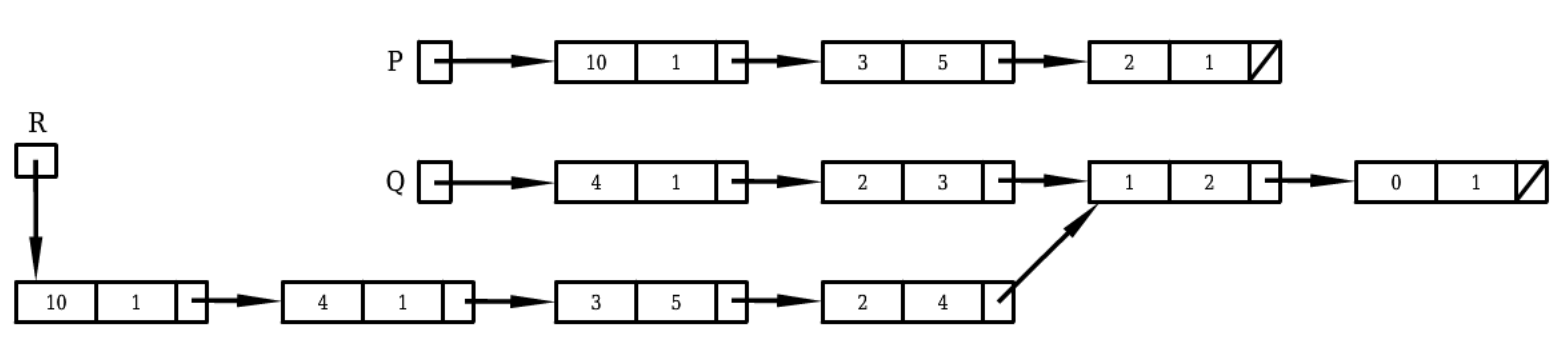
\includegraphics[width=12cm]{./img/Pic6.png}
\end{framed}
\caption{Сложение двух многочленов, представленных списками}
\end{figure}

\renewcommand{\figurename}{Алгоритм}

\newpage

\lhead{\small\textit{Решения упражнений}}
\rhead{161}

На рис. 6 видим схему памяти, представляющую три многочлена: $P =$ \linebreak $X^{10} + 5X^3 + X^2$, $Q = X^4 + 3X^2 + 2X + 1$ и $R = P + Q$, вычисленный с помощью предыдущего метода. Каждый элемент списка на этом рисунке представлен в виде тройки (степень, коэффициент, указатель). Этот метод реализован в алгоритме 18.

Построение списка, содержащего частичные последовательные результаты, осуществляется по возрастанию степеней. Следовательно, если один из списков исчерпался, нужно перевернуть промежуточный результат \linebreak прежде, чем присоединить хвост другого списка. Это делает подпрограмма \textit{Reverse\_Append}, которую можно поместить в пакет, разработанный в \linebreak упражнении 30. Эта функция реализована, начиная с примитивов управления списком: \textit{Head, Tail, Construct и Is\_Null}.

\begin{lstlisting} [language=C,
					basicstyle=\small,
					linewidth=14cm,
					mathescape=true,
					frame=none]
	$\textit{List}$ Reverse_Append($\textit{List}$ The_List, $\textit{List}$ And_The_List) {
		$\textit{List}$ x = The_List;
		$\textit{List}$ y = And_The_List;
		while (!Is_Null(x)) {
			y = Construct(x->Element, y);
			x = Tail(x);
		}
		return y;
	}
\end{lstlisting}

\begin{lstlisting} [language=C,
					basicstyle=\small,
					mathescape=true,
					caption=Сумма двух разреженных многочленов]
	R = Null_List;
	while (1) {
		if (Is_Null(Q)) return Reverse_Append(R, P);
		else if (Is_Null(P)) return Reverse_Append(R, Q);
		if (Head(Q)->Degree > Head(P)->Degree) {
			R = Construct(Head(Q), R);
			Q = Tail(Q);
		} else if (Head(P)->Degree > Head(Q)->Degree) {
			R = Construct(Head(P), R);
			P = Tail(P);
		} else {
			x = Head(P)->Coefficient + Head(Q)->Coefficient;
			if (x != 0)
				R = Construct(New_Element$\footnotemark$(Head(P)->Degree, x), R);
			P = Tail(P);
			Q = Tail(Q);
		}
	}
\end{lstlisting}

\footnotetext{\textit{New\_Element()} - "конструктор" объекта \textit{Element}. (Прим. редактора)}

Порядок многочлена есть его наименьшая степень, а его высота, обо- \linebreak

\newpage

\lhead{160}
\rhead{\small\textit{$I$ \quad Алгоритмика и программирование на языке Ада}}

\noindent
значаемая через $\sharp P$, — число ненулевых мономов в $P$. Если порядок $P$ больше порядка $Q$, то сложность алгоритма сложения прямо пропорциональна выражению:

\begin{center}
$\sharp P$ + число мономов многочлена $Q$ степени большей, чем порядок $P$.
\end{center}

\noindent
В этих вычислениях смешаны сложность просмотра списков и сложность вычисления арифметических операций — это вполне разумно в случае многочленов с небольшими целыми коэффициентами, но нереалистично, если арифметика коэффициентов более сложна.

\paragraph{32. Умножение многочленов, представленных списками} \mbox{}\\

Пусть $P = \sum a_i X^{\alpha_i}$, где $\alpha_i < \alpha_{i + 1}$ и $Q$ — два многочлена, которые требуется перемножить. Их произведение может вычисляться по формуле $R = \sum a_i X^{\alpha_i}Q$, если предполагается осуществлять умножение, следуя представлению $P$ в виде суммы одночленов. Легко видеть, что было бы удобно использовать функцию, реализующую умножение одночлена на многочлен. Эта функция легко и эффективно  реализуется, если воспользоваться более общей функцией, оперирующей списками таким образом, что на основании данного списка и некоторого преобразования его элементов она выдает новый список, полученный дублированием и преобразованием исходного списка. \newline

\textit{// here goes some code}

\end{document}
